\documentclass[tikz,border=10pt]{standalone}
\usepackage{amsmath}
\begin{document}
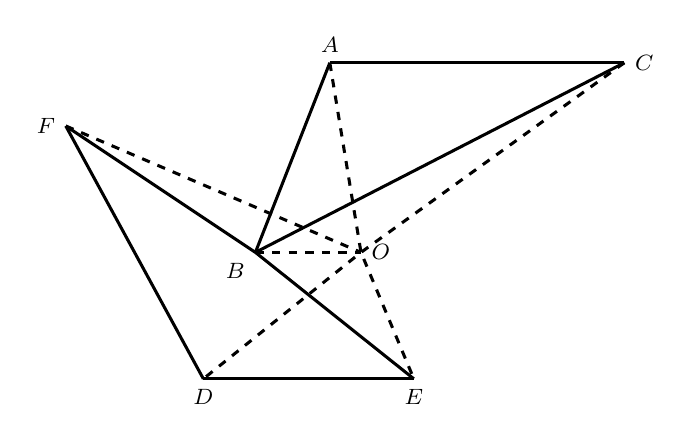
\begin{tikzpicture}[line width=1.1pt, line join=round, font=\fontsize{8.5}{10.2}\selectfont]
  % Points (scale s = 0.009445 cm/px, y flipped from 629 px height)
  \coordinate (A) at (4.345,4.987);
  \coordinate (C) at (8.085,4.987);
  \coordinate (F) at (0.992,4.184);
  \coordinate (B) at (3.400,2.579);
  \coordinate (O) at (4.741,2.579);
  \coordinate (D) at (2.739,0.973);
  \coordinate (E) at (5.412,0.973);

  % Solid segments
  \draw (A) -- (B);
  \draw (A) -- (C);
  \draw (B) -- (C);
  \draw (F) -- (D);
  \draw (D) -- (E);
  \draw (F) -- (B);
  \draw (B) -- (E);

  % Dashed segments
  \draw[dashed] (A) -- (O) -- (E);
  \draw[dashed] (C) -- (O) -- (D);
  \draw[dashed] (F) -- (O);
  \draw[dashed] (B) -- (O);

  % Labels
  \node[above] at (A) {$A$};
  \node[right] at (C) {$C$};
  \node[left] at (F) {$F$};
  \node[below left] at (B) {$B$};
  \node[right] at (O) {$O$};
  \node[below] at (D) {$D$};
  \node[below] at (E) {$E$};
\end{tikzpicture}
\end{document}